 
%% bare_conf.tex
%% V1.3
%% 2007/01/11
%% by Michael Shell
%% See:
%% http://www.michaelshell.org/
%% for current contact information.
%%
%% This is a skeleton file demonstrating the use of IEEEtran.cls
%% (requires IEEEtran.cls version 1.7 or later) with an IEEE conference paper.
%%
%% Support sites:
%% http://www.michaelshell.org/tex/ieeetran/
%% http://www.ctan.org/tex-archive/macros/latex/contrib/IEEEtran/
%% and
%% http://www.ieee.org/

%%************************************************************************
%% Legal Notice:
%% This code is offered as-is without any warranty either expressed or
%% implied; without even the implied warranty of MERCHANTABILITY or
%% FITNESS FOR A PARTICULAR PURPOSE! 
%% User assumes all risk.
%% In no event shall IEEE or any contributor to this code be liable for
%% any damages or losses, including, but not limited to, incidental,
%% consequential, or any other damages, resulting from the use or misuse
%% of any information contained here.
%%
%% All comments are the opinions of their respective authors and are not
%% necessarily endorsed by the IEEE.
%%
%% This work is distributed under the LaTeX Project Public License (LPPL)
%% ( http://www.latex-project.org/ ) version 1.3, and may be freely used,
%% distributed and modified. A copy of the LPPL, version 1.3, is included
%% in the base LaTeX documentation of all distributions of LaTeX released
%% 2003/12/01 or later.
%% Retain all contribution notices and credits.
%% ** Modified files should be clearly indicated as such, including  **
%% ** renaming them and changing author support contact information. **
%%
%% File list of work: IEEEtran.cls, IEEEtran_HOWTO.pdf, bare_adv.tex,
%%                    bare_conf.tex, bare_jrnl.tex, bare_jrnl_compsoc.tex
%%*************************************************************************

% *** Authors should verify (and, if needed, correct) their LaTeX system  ***
% *** with the testflow diagnostic prior to trusting their LaTeX platform ***
% *** with production work. IEEE's font choices can trigger bugs that do  ***
% *** not appear when using other class files.                            ***
% The testflow support page is at:
% http://www.michaelshell.org/tex/testflow/



% Note that the a4paper option is mainly intended so that authors in
% countries using A4 can easily print to A4 and see how their papers will
% look in print - the typesetting of the document will not typically be
% affected with changes in paper size (but the bottom and side margins will).
% Use the testflow package mentioned above to verify correct handling of
% both paper sizes by the user's LaTeX system.
%
% Also note that the "draftcls" or "draftclsnofoot", not "draft", option
% should be used if it is desired that the figures are to be displayed in
% draft mode.
%
\documentclass[10pt, conference, compsocconf]{IEEEtran}
% Add the compsocconf option for Computer Society conferences.
%
% If IEEEtran.cls has not been installed into the LaTeX system files,
% manually specify the path to it like:
% \documentclass[conference]{../sty/IEEEtran}





% Some very useful LaTeX packages include:
% (uncomment the ones you want to load)


% *** MISC UTILITY PACKAGES ***
%
%\usepackage{ifpdf}
% Heiko Oberdiek's ifpdf.sty is very useful if you need conditional
% compilation based on whether the output is pdf or dvi.
% usage:
% \ifpdf
%   % pdf code
% \else
%   % dvi code
% \fi
% The latest version of ifpdf.sty can be obtained from:
% http://www.ctan.org/tex-archive/macros/latex/contrib/oberdiek/
% Also, note that IEEEtran.cls V1.7 and later provides a builtin
% \ifCLASSINFOpdf conditional that works the same way.
% When switching from latex to pdflatex and vice-versa, the compiler may
% have to be run twice to clear warning/error messages.






% *** CITATION PACKAGES ***
\usepackage{amsmath}
\usepackage{fullpage}
\usepackage[utf8]{inputenc}
\usepackage{mathtools}
\usepackage{amssymb}
\usepackage{graphicx}
\graphicspath{{C:\Users\Manmohan\Documents\GitHub\research}}




% *** GRAPHICS RELATED PACKAGES ***
% 
\ifCLASSINFOpdf
  % \usepackage[pdftex]{graphicx}
  % declare the path(s) where your graphic files are
  % \graphicspath{{../pdf/}{../jpeg/}}
  % and their extensions so you won't have to specify these with
  % every instance of \includegraphics
  % \DeclareGraphicsExtensions{.pdf,.jpeg,.png}
\else
 
\fi



% correct bad hyphenation here
\hyphenation{op-tical net-works semi-conduc-tor}


\begin{document}
%
% paper title
% can use linebreaks \\ within to get better formatting as desired
\title{Replication of Data Placement for Uncertain Scheduling}


% author names and affiliations
% use a multiple column layout for up to two different
% affiliations

\author{\IEEEauthorblockN{Manmohan Chaubey, Erik Saule }
\IEEEauthorblockA{Department of Computer Science\\
 University of North Carolina at Charlotte\\
 Charlotte, USA\\
 Email: mchaubey@uncc.edu, esaule@uncc.edu}

}





% make the title area
\maketitle


\begin{abstract}
The abstract goes here. DO NOT USE SPECIAL CHARACTERS, SYMBOLS, OR MATH IN YOUR TITLE OR ABSTRACT.

\end{abstract}

\begin{IEEEkeywords}
component; formatting; style; styling;

\end{IEEEkeywords}


% For peer review papers, you can put extra information on the cover
% page as needed:
% \ifCLASSOPTIONpeerreview
% \begin{center} \bfseries EDICS Category: 3-BBND \end{center}
% \fi
%
% For peerreview papers, this IEEEtran command inserts a page break and
% creates the second title. It will be ignored for other modes.
\IEEEpeerreviewmaketitle

\section{Introduction}

Many real world scheduling problems related to task allocation in parallel machines are uncertain in nature. This fact makes the class of problem  known as 'scheduling with uncertainty' or 'robust' scheduling an important and most studied problem in Scheduling.  Often in  scheduling models the exact value of parameters such as processing times of tasks, are not known initially,   but they have a range outside which their values cannot  lie.  This paper draws qualitative analysis of the effect of replication in data placement for uncertain scheduling with inexact processing time of a task. Thus  our research brings two area of scheduling problem together i.e. task uncertainty and data placement.  The scheduling problem related to data placement and task allocation is common in heterogeneous systems and often dealt with common approach.  The objective of our reseach  is to propose an optimization approach that takes into account  effective data placement using replication to schedule  tasks in the environment where processing time of tasks are not known exactly but they can be estimated based on some pre estimated values.

Data placement technique can be useful in the scenario of uncertain processing times of tasks. Effective data placement using replication strategy allows better load balancing and hence reduces turnaround job time.   This paper is important in the sense that it proposes different models depending upon different scenarios and compares them based on approximation ratio and replication they allow.  Replication strategy that allows to place data in a wisely manner  offers a faster access to files required by  jobs, hence increases the job execution’s performance. Replication helps in load balancing but it have certain cost attached with it as it usually increases resource usage\cite{IEEEhowto:wang}.  The paper deals with this problem and chooses the scenario in which replication is beneficial. 


There is very less literature available for scheduling with estimated processing time of a task.  Most of the literature till now focuses on job size estimation with small error.  Very less work is done which focuses on coping with less restrictive estimation for task size and which analyzes the effect of estimation on scheduling quantitatively.   Wierman and Nuyens \cite{IEEEhowto:Wierman} introduce $ \xi-SMART$ as classification to understand size based policies and draw analytical co-relation between response time and estimated job size in single server problem. \cite{IEEEhowto:Matteo} provides insight into scheduling behavior when estimation error is present and proposes FSPE+PS based policy to cope with this problem.
 
Size estimation based policies are widely used in practicality in the area of MapReduce and Hadoop. \cite{IEEEhowto:Wolf} \cite{IEEEhowto:Pastorelli} proposes schedulers which provides robustness in scheduling against uncertain Job Size. \cite{IEEEhowto:Canon} provides scheduling heuristics that optimizes both makespan and robustness in scheduling task graph on heterogenous system.

In literature uncertainty problems are also viewed as sensitivity analysis and purturbations in processing time of a task. \cite{IEEEhowto:Gatto} derives bounds on competitive ratio of Graham’s online algorithm in scenario where processing times of jobs either increase or decrease arbitrarily due to pertured processing times of tasks.

\cite{IEEEhowto:Guinand} presents sensitivity analysis for scheduling trees with communication
delays on two identical machines.  Wagelmans give supporting evidence for the notion  that a good performance of an algorithms  is identical with a high degree of sensitivity \cite{IEEEhowto:Wagelmans}. 

The remaining of the paper is organized as follows:we describe system model and notatins in section 2. Sections 3-5 describes different problem models- 1)No replications, 2)replication is done everywhere and 3)replication is done within a group. The respective sections describe derivation of comptetitave ratios for each of these models. Section 6 summarises the 3 models and based on experimental results.  

\section{Problem Definition}
% no \IEEEPARstart
We have set $J$ of $n$ jobs which need to be scheduled to set $M$ of $m$ machines such that makespan, $C_{max}$ is minimized.   $C_{max}^{*}$ denotes optimal makespan of a schedule $S$.   We are considering the problems where the scheduler do not know the processing time of a task exactly before it completes, but we have some estimation of the processing time of a task before it is  assigned to a processor. We know that the actual processing time of a task $i$ is between $\frac{1}{\alpha}$and $\alpha$ times of its estimated processing time. $p_i$ denotes the actual processing time and $\tilde {p_i}$ denotes
estimated processing time for the task $i$.  We have this estimate:\\
\begin{equation} 
\frac{1}{\alpha}\leq \frac{p_{i}}{\tilde{p}_{i}}\leq \alpha
\end{equation}\\

[Note:give justification ]


We consider various problem models  incorporating the above mentioned scenario of uncertain processing times of tasks with an estimate. Depending upon  a problem model the scheduling is done in two phases or just in one phase. In Phase 1, we allocate tasks to certain processors or group of processors depending upon a problem model.  Phase 1 chooses where data to be  replicated using estimated processing time $\tilde p_i $, for each of the task $i$. Phase 1 takes $\tilde{p_i}$, $m$ and $\alpha$ as input and outputs set of machines, $M_j \subseteq M $ where a task $j$ can be scheduled or is replicated. Phase 2 takes output of phase 1 as input and outputs set of task assigned to a machine $i$, $E_i \subseteq J$.   In Phase 2, we choose actual schedule with semi-clairvoyant algorithm which uses only approximate knowledge of initial processing time, and after scheduling the task the actual $p_i$ is known.  With  objective to find schedule which minimizes makespan, we investigate greedy algorithms for each of the problem models and prove their comptetitive ratios. \\

We have used  Graham's List Scheduling (LS) and Largest Processing Time (LPT) algorithms to derive approximation ratios in different scenarios. The LS algorithm takes tasks one at a time and assign  it to the processor having least load at that time. LS is 2-approximation algorithm and is widely used in online scheduling problems.  The LPT sorts tasks in decreasing order of processing time and assign them one at a time in this order to the processor with the smallest current load. The LPT algorithm have worst case performance ratio as $4/3-1/(3m) $ in offline setting
. Depending upon which among these two algorithms suits more for a problem model we have used these algorithms accordingly. 

\section{Model 1: No replication} 
In this problem model we have considered  situation where each task is restricted to be scheduled on only one machine, i.e. $|M_j|=1$.  We have a set $J$ of $ n$ jobs, and a set $M$ of $m$ machines.  Let $f : J \leftarrow M$ be a function that assigns each job to exactly one machine. Let us denote $E_{i}$ as the set tasks which is assigned to a machine $i$.  The restriction that each task can be scheduled to only one machine restrict the problem constrution to phase one only. There is no replication of tasks in this model.\\
\\

We have  considered List scheduling and Longest processing time algorithms and have  assigned each task on machine on which they are restricted to.   Based on the estimated processing times of  tasks loaded on each machine we will derive makespan. \\                                                                                                                                                                                                                                                                                                                                                                                                                                                                                                                                                                                                                                                                                                                                                                                                                                                                                                                                                                                                                                                                                                                                                                                                                                                                                                                                                                                                                                                                                                                                                                                                                                                                                                                                                                                                                                                                                                                                                                                                                                                                                                                                                                                                                                                                                                                                                                                                                                                                                                                                                                                                                                                                                                                                                                                                                                                                                                                                                                                                                                                                                                                                                                                                                                                                                                                                                                                                                                                                                                                                                                                                                                                                                                                                                                                                                                                                                                                                                                                                                                                                                                                                                                                                                                                                                                                                                                                                                                                                                                                                                                                                                                                                                                                                                                                                                                                                                                                                                                                                                                                                                                                                                                                                                                                                                                                                                                                                                                                                                                                                                                                                                                                                                                                                                                                                                                                                                                                                                                                                                                                                                                                                                                                                                                                                                                                                                                                                                                                                                                                                                                                                                                                                                                                                                                                                                                                                                                                                                                                                                                                                                                                                                                                                                                                                                                                                                                                                                                                                                                                                                                                                                                                                                                                                                                                                                                                                                                                                                                                                                                                                                                                                                                                                                                                                                                                                                                                                                                                                                                                                                                                                                                                                                                                                                                                                                                                                                                                                                                                                                                                                                                                                                                                                                                                                                                                                                                                                                                                                                                                                                                                                                                                                                                                                                                                                                                                                                                                                                                                                                                                                                                                                                                                                                                                                                                                                                                                                                                                                                                                                                                                                                                                                                                                                                                                                                                                                                                                                                                                                                                                                                                                                                                                                                                                                                                                                                                                                                                                                                                                                                                                                                                                                                                                                                                                                                                                                                                                                                                                                                                                                                                                                                                                                                                                                                                                                                                                                                                                                                                                                                                                                                                                                                                                                                                                                                                                                                                                                                                                                                                                                                                                                                                                                                                                                                                                                                                                                                                                                                                                                                                                                                                                            
\subsection{Lower Bound}
\textbf{Thoerem 1.1:} There is no online algorithm having competitive  ratio better than $\alpha^{2} $.\\
\textbf{Proof:}  We  use adversary technique to prove that there is no online algorithm having competitive  ratio better than $\alpha^{2} $\\
 
 Let us consider an instance in which total tasks be $\lambda m$ with $\tilde{p_i}=1$. After scheduling let the most loaded machine $j$ have $B$ tasks. Obviously, $B \geq \lambda$. In phase 2 the adversary  increases the tasks on $j$ by $\alpha$ and decreases the other tasks by $\alpha$. So, $ C_{max}$ = $\alpha B$ and ${C^{*}_{max}}\geq \frac{\alpha B + \frac{1}{\alpha }  (\lambda  m - B) }{m}$. We have,
 
 \begin{equation}\nonumber
\frac{C_{max}}{C^{*}_{max}}\leq \frac{\alpha^{2} B m }{\alpha^{2} B + \lambda m - B}=\frac{\alpha^{2}  m }{\alpha^{2}  + \frac{\lambda m}{B}  - 1}
 \end{equation} 
  From above expression it is clear that smaller the value of $B$, the value of $\frac{C_{max}}{C^{*}_{max}}$ decreases.  Irrespective of the value of $\lambda$,for $B= \lambda$ the value of expression would be minimum and is equal to $\frac{\alpha^{2}  m }{\alpha^{2}  + m  - 1}$. When $m$ tends to $\infty$ the expression equals $\alpha^2$. So, any algorithm   cannot give competitive ratio better than $\alpha^2$.
  
  \begin{figure}[htp]
  \centering
  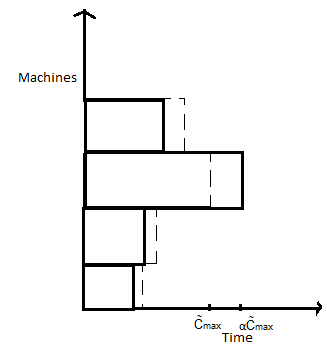
\includegraphics[width= 8 cm]{fig1}
  \caption{ Model 1  }
  \label{fig:rara}
  \end{figure}
 
 
 
\subsection{Algorithm}



\textbf{Theorem 1.2:} Using LPT the competitive ratio is $ \frac{2\alpha^{2}m}{2\alpha^{2}+ m-1}$.

\textbf{Proof:} In this problem model we are assigning tasks to processors using LPT in offline mode using non-increasing order of estimated processing times of tasks.

 


 
\begin{equation}
\tilde C_{max}\leq  \frac{\sum{\tilde p_j + (m-1) \tilde p_l} }{m}
\end{equation}

where $\tilde C_{max}$ is makespan considering estimated processing  times  of tasks.  Also actual processing time  $C_{max}$ must be smaller the $\alpha\tilde C_{max}$, we have \\

\begin{equation}
 C_{max}\leq \alpha \tilde C_{max}\leq \alpha [\frac{\sum{\tilde p_j + (m-1) \tilde p_l} }{m}] 
\end{equation} 

Considering the worst case situation the processor with $\tilde C_{max}$ will see its tasks increase by $\alpha$  and the load on the  rest of the processors will by shrink  $\frac{1}{\alpha}$.  The argument behind this statement is that greater the value of ratio $\frac{C_{max}}{\sum{p_j}}$, the algorithm will give bad approximation. So increasing the load on the machine which have $C_{max} $ and decrasing the rest of the load on other processors will reach worst case scenario. So the total actual processing time is given by the  following equation.
 \begin{equation}
 \sum {p_j} = \frac{\tilde p_j- \tilde C_{max}}{\alpha} + \alpha \tilde C_{max}
 \end{equation}
 
 Also the actual optimal makespan have following constraint
 \begin{equation}\nonumber 
C_{max}^{*}\geq \frac{\sum {p_j}}{m}
\end{equation}

Substituiting for  $ \sum {p_j}$, we have

 \begin{equation}\nonumber 
 m C_{max}^{*}\geq \frac{\tilde p_j- \tilde C_{max}}{\alpha} + \alpha \tilde C_{max}
 \end{equation}
 
\begin{equation}\nonumber 
\Rightarrow m C_{max}^{*}\geq \frac{\tilde p_j-[\frac{\sum{\tilde p_j + (m-1) \tilde p_l }}{m}]} {\alpha} + {C_{max}}
\end{equation}

\begin{equation}\nonumber
\Rightarrow m C_{max}^{*}\geq \frac{m-1}{\alpha m} [\sum \tilde p_j-\tilde p_l] + {C_{max}}
 \end{equation}

By the property of LPT $\sum \tilde p_j-\tilde p_l \geq m (\tilde C_{max}-\tilde p_l)$, putting this we have,\\
\begin{equation}\nonumber 
 m C_{max}^{*}\geq \frac{m-1}{\alpha } \left[\tilde C_{max}-\tilde p_l\right] + {C_{max}}
 \end{equation}
\begin{equation}\nonumber
\Rightarrow m C_{max}^{*}\geq \frac{m-1}{\alpha } \left[\tilde C_{max}-\frac{\tilde C_{max}}{2}\right] + {C_{max}}
\end{equation}
\begin{equation}\nonumber
\Rightarrow m C_{max}^{*}\geq \frac{m-1}{2\alpha } \left[\frac{C_{max}} {\alpha} \right]+ {C_{max}}
\end{equation}
\begin{equation}\nonumber
\Rightarrow m C_{max}^{*}\geq \left[\frac{m-1}{2\alpha^{2} } +1\right]{C_{max}}
\end{equation}
\begin{equation}\nonumber
\Rightarrow \frac{C_{max}}{C_{max}^{*}}\leq \frac{2\alpha^{2}m}{2\alpha^{2}+ m-1}
\end{equation}



\section{Model 2: replication is done everywhere}
In this problem model we consider no restrictaion on task assignment.  In the first phase task are replicated everywhere i.e. $\forall j, |M_{j}|=|M|$.  All tasks are allowed to replicate everywhere There are $ n$ tasks which need to be  assigned to $m$ processors. In the second phase we   simplly use the  Largest Processing Time algorithm (LPT) using estimated processing times of tasks in non-increasing order as input.  \\




\textbf{Lemma 2.1:} $C_{max}^{*} \geq {\frac{2}{\alpha^{2}}} p_l $  when there are at least two tasks in the machine to which the last task, $l$ is scheduled.

\textbf{Proof:} Suppose $l$ be the last task with estimated processing time $\tilde p_l$. Suppose
there are at least two tasks in the machine in which $l$ is assigned including $l$. Let
$C_{max}$ be the be makespan of the schedule and $C_{max}^{*}$ be the optimal makespan.\\

As there is at least one task $j$ before $l$ in the machine to which $l$ is
assigned, we have
\begin{equation}\nonumber
C_{max}^{*}\geq p_l + p_j
\end{equation}



As actual processing time of a task must be greater than $\frac{1}{\alpha}$ times of its estimated value, we have
\begin{equation}\nonumber 
C_{max}^{*} \geq \frac{1}{\alpha}\tilde p_l +  \frac{1}{\alpha} \tilde p_j 
\end{equation}
\\
As $j$ is scheduled before $l$ using LPT on estimated values of processing times,  $\tilde p_j\geq   \tilde p_l$ holds true for tasks $l$ and $j$.  Using this, we have\\

\begin{equation}\nonumber
 C_{max}^{*} \geq \frac{2}{\alpha}\tilde p_l
 \end{equation}
\begin{equation}
\Rightarrow C_{max}^{*} \geq {\frac{2}{\alpha^{2}}} p_l  \end{equation}


\textbf{Theorem 2.1:} $\frac{C_{max}}{C_{max}^{*}} \leq 1 + (\frac{m-1}{m})\frac{\alpha^{2}}{2}$\\
\\
\textbf{Proof:} The optimal makespan, $C_{max}^{*}$ must be at least equal to the average load on the $m$ machines. We have\\
\begin{equation}
C_{max}^{*}\geq\frac{\sum p_j}{m}
\end{equation}

By the property of LPT the load on each machine $i$ is greater than the load on the machine which reach $C_{max}$ before the last task $l$ is scheduled. So for each machine $i$, $C_{max} \leq  \sum_{j \in E_i}^{}{p_j} + p_l$ holds true.  Summing for all the machines we have\\

\begin{equation}\nonumber 
mC_{max} \leq  \sum {p_j} + (m-1)p_l
\end{equation}

\begin{equation}
C_{max} \leq  \frac{\sum {p_j}}{m} + \frac{(m-1)}{m}p_l
\end{equation}
\\
Using (6) and (7), we have\\

\begin{equation}\nonumber
\frac{C_{max}}{C_{max}^{*}} \leq 1 + {\frac{m-1}{m}}\left(\frac{p_l}{C_{max}^{*}}\right)
\end{equation}

As $C_{max}^{*} \geq {\frac{2}{\alpha^{2}}} p_l $, We have \\

\begin{equation}\nonumber
\frac{C_{max}}{C_{max}^{*}} \leq 1 + \left(\frac{m-1}{m}\right)\frac{\alpha^{2}}{2}
\end{equation}
Hence the theorem follows.   \\                            



\section{Model 3: Replication in groups}
In this model the first phase is in offline mode and each task is pre-assigned to a particular  group of processors. In the second phase the tasks are scheduled  within the group they are assigned to in first phase.   We have a set $J$ of $ n$ jobs.  There are $k$ groups and size of each group is equal and have $m/k$ processors within each group.  We have considered task allocation in a group such that each task can be assigned to only one group, i.e. $\forall j$, $|M_j|= m/k$.  In phase 2  each task is scheduled to a particular processor within the group it was allocated in phase 1.  We propose  List Sheduling algorithm in both the phases. In phase 1 using LS we pre-assign the tasks in different groups.  In phase 2 we use online LS to schedule tasks to processors within each group.

\begin{figure*}[htp]
\centering
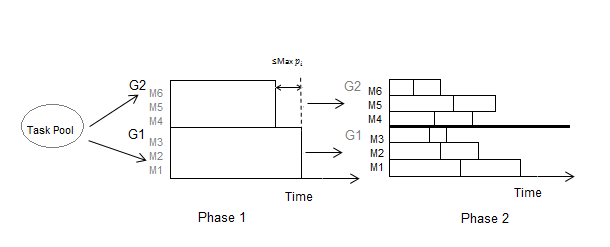
\includegraphics[width= 16 cm]{fig2}
\caption{Model 3}
\label{fig:Model 3}
\end{figure*}





\textbf{Theorem 3.1:} When the number of groups is $k$ the approximation ratio is $  \frac{k\alpha^{2}}{\alpha^{2}+k-1}[1+ {\frac{k-1}{m}} ]+ {\frac{m-k}{m}}   $ \\
\\
\textbf{Proof:} 
  We have $k$ groups of $m/k$ machines. We have restriction that each task can be assigned to only one of these groups. In Phase 1, each task is assigned to different groups. In Phase 2, tasks are scheduled online within repective group.

Let us consider  that $ C_{max}$ comes from group  $G1$. Also, taking the property of List Scheduling that the load difference between any two groups cannot be greater than the largest task. So, for any group $Gl \neq G1$, We have\\

\begin{equation}{\nonumber}
|\sum_{i \in G1 }^{}{\tilde p_{i}}- \sum_{i \in Gl }^{}{\tilde p_{i}}| \leq {max_{i \in T}}{\tilde p_{i}}\end{equation}  \hspace*{15pt}   for all, $l = 2,3,...,k$ \\

Adding for all values of $l$, We have \\

\begin{equation}{\nonumber}
|(k-1)\sum_{i \in G1 }^{}{\tilde p_{i}}- \sum_{l=2}^{k}\sum_{i \in Gl }^{}{\tilde p_{i}}| \leq (k-1) {max_{i \in T}}{\tilde p_{i}}
\end{equation}

\begin{equation}{\nonumber}
\Rightarrow \sum_{l=2}^{k}\sum_{i \in Gl }^{}{\tilde p_{i}} \geq (k-1)[\sum_{i \in G1 }^{}{\tilde p_{i}}- {max_{i \in T}}{\tilde p_{i}}]
\end{equation}



As the actual processing time of tasks  can vary within a factor $\alpha$ and $\frac{1}{\alpha}$ of their estimated processing time, the following inequality holds\\
\\
\begin{equation}{\nonumber}
 \alpha\sum_{l=2}^{k}\sum_{i \in Gl }^{}{{p_{i}}} \geq (k-1)[\frac{1}{\alpha}\sum_{i \in G1 }^{}{{p_{i}}}- \alpha {max_{i \in T}}{{p_{i}}}]
\end{equation}
\begin{equation}
\sum_{l=2}^{k}\sum_{i \in Gl }^{}{{p_{i}}} \geq (k-1)[\frac{1}{\alpha^{2}}\sum_{i \in G1 }^{}{{p_{i}}}-  {max_{i \in T}}{{p_{i}}}]
\end{equation}

In phase 2, We are applying LS on online mode. We assume that $C_{max}$ comes from $G1$. Using LS property we can write,

\begin{equation}
 C_{max} \leq \frac{\sum_{i \in G1 }^{}{{p_{i}}}}{m/k} + {\frac{m/k-1}{m/k}} p_{max} 
\end{equation}
\\

Also, $C_{max}^{*}$ must be greater than the average of the  loads on  machines.\\

\begin{equation}{\nonumber}
C_{max}^{*} \geq  \frac{\sum_{i \in T }^{}{{p_{i}}}}{m}
\end{equation}

\begin{equation}
{\nonumber}\Rightarrow C_{max}^{*} \geq  \frac{\sum_{i \in G1 }^{}{{p_{i}}}+ \sum_{l=2}^{k}\sum_{i \in Gl }^{}{{p_{i}}}}{m}
\end{equation}




from (11), we derive\\

\begin{equation}{\nonumber}
\Rightarrow C_{max}^{*} \geq  \frac{\sum_{i \in G1 }^{}{{p_{i}}}+ (k-1)\left[\frac{1}{\alpha^{2}}\sum_{i \in G1 }^{}{{p_{i}}}-  {max_{i \in T}}{{p_{i}}}\right]}{m}
\end{equation}

\begin{equation}{\nonumber}
\Rightarrow m\alpha^{2}C_{max}^{*} + \alpha^{2} (k-1){max_{i \in T}}{{p_{i}}} \geq  \alpha^{2}\sum_{i \in G1 }^{}{{p_{i}}}+ (k-1)\sum_{i \in G1 }^{}{{p_{i}}} 
\end{equation}
\begin{equation}
\Rightarrow\frac{\alpha^{2}}{\alpha^{2}+k-1}\left[m C_{max}^{*}+(k-1) {max_{i \in T}}{{p_{i}}}\right] \geq \sum_{i \in G1 }^{}{{p_{i}}}  
\end{equation}
\\
Using (12) and (13), We have

\begin{equation}{\nonumber}
C_{max} \leq \frac{k\alpha^{2}}{\alpha^{2}+k-1}\left[ C_{max}^{*}+\frac{(k-1)}{m} {max_{i \in T}}{{p_{i}}}\right] + {\frac{m/k-1}{m/k}} p_{max} 
\end{equation}
 As $C_{max}^{*}\geq {{max_{i \in T}}{p_{i}}}\geq p_{max}$, we have\\
\begin{equation}{\nonumber}
 C_{max} \leq \frac{k\alpha^{2}}{\alpha^{2}+k-1}\left[ C_{max}^{*}+ {\frac{k-1}{m}}{C_{max}^{*}}\right] + {\frac{m-k}{m}} C_{max}^{*} \end{equation} \\
 

 
 So we have approximation ratio,\\
 \begin{equation}{\nonumber}
\frac{C_{max}}{C_{max}^{*}} \leq \frac{k\alpha^{2}}{\alpha^{2}+k-1}\left[1+ {\frac{k-1}{m}} \right]+ {\frac{m-k}{m}} \end{equation}



\textbf{Corollary 3.1:} When the number of groups is $2$ the approximation ratio is $ 1+ \frac{2}{1+\alpha^{2}} (\alpha^2-\frac{1}{m})  $ \\







% An example of a floating figure using the graphicx package.
% Note that \label must occur AFTER (or within) \caption.
% For figures, \caption should occur after the \includegraphics.
% Note that IEEEtran v1.7 and later has special internal code that
% is designed to preserve the operation of \label within \caption
% even when the captionsoff option is in effect. However, because
% of issues like this, it may be the safest practice to put all your
% \label just after \caption rather than within \caption{}.
%
% Reminder: the "draftcls" or "draftclsnofoot", not "draft", class
% option should be used if it is desired that the figures are to be
% displayed while in draft mode.
%
%\begin{figure}[!t]
%\centering
%\includegraphics[width=2.5in]{myfigure}
% where an .eps filename suffix will be assumed under latex, 
% and a .pdf suffix will be assumed for pdflatex; or what has been declared
% via \DeclareGraphicsExtensions.
%\caption{Simulation Results}
%\label{fig_sim}
%\end{figure}

% Note that IEEE typically puts floats only at the top, even when this
% results in a large percentage of a column being occupied by floats.


% An example of a double column floating figure using two subfigures.
% (The subfig.sty package must be loaded for this to work.)
% The subfigure \label commands are set within each subfloat command, the
% \label for the overall figure must come after \caption.
% \hfil must be used as a separator to get equal spacing.
% The subfigure.sty package works much the same way, except \subfigure is
% used instead of \subfloat.
%
%\begin{figure*}[!t]
%\centerline{\subfloat[Case I]\includegraphics[width=2.5in]{subfigcase1}%
%\label{fig_first_case}}
%\hfil
%\subfloat[Case II]{\includegraphics[width=2.5in]{subfigcase2}%
%\label{fig_second_case}}}
%\caption{Simulation results}
%\label{fig_sim}
%\end{figure*}
%
% Note that often IEEE papers with subfigures do not employ subfigure
% captions (using the optional argument to \subfloat), but instead will
% reference/describe all of them (a), (b), etc., within the main caption.


% An example of a floating table. Note that, for IEEE style tables, the 
% \caption command should come BEFORE the table. Table text will default to
% \footnotesize as IEEE normally uses this smaller font for tables.
% The \label must come after \caption as always.
%
%\begin{table}[!t]
%% increase table row spacing, adjust to taste
%\renewcommand{\arraystretch}{1.3}
% if using array.sty, it might be a good idea to tweak the value of
% \extrarowheight as needed to properly center the text within the cells
%\caption{An Example of a Table}
%\label{table_example}
%\centering
%% Some packages, such as MDW tools, offer better commands for making tables
%% than the plain LaTeX2e tabular which is used here.
%\begin{tabular}{|c||c|}
%\hline
%One & Two\\
%\hline
%Three & Four\\
%\hline
%\end{tabular}
%\end{table}


% Note that IEEE does not put floats in the very first column - or typically
% anywhere on the first page for that matter. Also, in-text middle ("here")
% positioning is not used. Most IEEE journals/conferences use top floats
% exclusively. Note that, LaTeX2e, unlike IEEE journals/conferences, places
% footnotes above bottom floats. This can be corrected via the \fnbelowfloat
% command of the stfloats package.



\section{Summary}

The Table \ref{tab:template} summarizes the results in term of approximation ratio given by the three models.

\begin{table}[ht]
\centering
\begin{tabular}{|l|c|c|c|c|c|}
\hline
Replication & Approximation ratio  \\
\hline
$|M_j|=1$ & $\frac{C_{max}}{C_{max}^{*}}\leq \frac{2\alpha^{2}m}{2\alpha^{2}+ m-1}$ [Th. 1.2]  \\
 & No approximation better than $\alpha^2$ [Th. 1.1]   \\

\hline
$|M_j|=|M|$ & $\frac{C_{max}}{C_{max}^{*}} \leq 1 + (\frac{m-1}{m})\frac{\alpha^{2}}{2}$ [Th. 2.1]  \\

 \hline
 
 $|M_j|= m/k $ & $\frac{C_{max}}{C_{max}^{*}} \leq \frac{k\alpha^{2}}{\alpha^{2}+k-1}\left[1+ {\frac{k-1}{m}} \right]+ {\frac{m-k}{m}}$ [Th. 3.1]  \\
  & $\frac{C_{max}}{C_{max}^{*}} \leq  1+ \frac{2}{1+\alpha^{2}} \left(\alpha^2-\frac{1}{m}\right)$ when $k=2$ [Col. 3.1]   \\
  
  \hline
 \end{tabular}
\caption{Summary Table}
\label{tab:template}
\end{table}


The figure \ref{fig:graph} shows ratio- replication graphs for each of the models for different values of $ \alpha$.  We vary the value of $\alpha$ while keeping the number of machines fixed, $m=210$. For replication everywhere scenario the number of replication is full and is always equal to total number of machines.  For no replication scenario the approximation ratio is fixed for each value of $\alpha$.  For the model where replication is allowed within the group the approximation ratio decreases significantly for small replication. We observe that after a significant number of replications the ratio is not much improved further. 


\begin {figure}
\begin{center}
% GNUPLOT: LaTeX picture
\setlength{\unitlength}{0.240900pt}
\ifx\plotpoint\undefined\newsavebox{\plotpoint}\fi
\sbox{\plotpoint}{\rule[-0.200pt]{0.400pt}{0.400pt}}%
\begin{picture}(826,590)(0,0)
\sbox{\plotpoint}{\rule[-0.200pt]{0.400pt}{0.400pt}}%
\put(171.0,131.0){\rule[-0.200pt]{4.818pt}{0.400pt}}
\put(151,131){\makebox(0,0)[r]{ 1.6}}
\put(745.0,131.0){\rule[-0.200pt]{4.818pt}{0.400pt}}
\put(171.0,177.0){\rule[-0.200pt]{4.818pt}{0.400pt}}
\put(151,177){\makebox(0,0)[r]{ 1.7}}
\put(745.0,177.0){\rule[-0.200pt]{4.818pt}{0.400pt}}
\put(171.0,224.0){\rule[-0.200pt]{4.818pt}{0.400pt}}
\put(151,224){\makebox(0,0)[r]{ 1.8}}
\put(745.0,224.0){\rule[-0.200pt]{4.818pt}{0.400pt}}
\put(171.0,270.0){\rule[-0.200pt]{4.818pt}{0.400pt}}
\put(151,270){\makebox(0,0)[r]{ 1.9}}
\put(745.0,270.0){\rule[-0.200pt]{4.818pt}{0.400pt}}
\put(171.0,317.0){\rule[-0.200pt]{4.818pt}{0.400pt}}
\put(151,317){\makebox(0,0)[r]{ 2}}
\put(745.0,317.0){\rule[-0.200pt]{4.818pt}{0.400pt}}
\put(171.0,363.0){\rule[-0.200pt]{4.818pt}{0.400pt}}
\put(151,363){\makebox(0,0)[r]{ 2.1}}
\put(745.0,363.0){\rule[-0.200pt]{4.818pt}{0.400pt}}
\put(171.0,410.0){\rule[-0.200pt]{4.818pt}{0.400pt}}
\put(151,410){\makebox(0,0)[r]{ 2.2}}
\put(745.0,410.0){\rule[-0.200pt]{4.818pt}{0.400pt}}
\put(171.0,456.0){\rule[-0.200pt]{4.818pt}{0.400pt}}
\put(151,456){\makebox(0,0)[r]{ 2.3}}
\put(745.0,456.0){\rule[-0.200pt]{4.818pt}{0.400pt}}
\put(171.0,503.0){\rule[-0.200pt]{4.818pt}{0.400pt}}
\put(151,503){\makebox(0,0)[r]{ 2.4}}
\put(745.0,503.0){\rule[-0.200pt]{4.818pt}{0.400pt}}
\put(171.0,549.0){\rule[-0.200pt]{4.818pt}{0.400pt}}
\put(151,549){\makebox(0,0)[r]{ 2.5}}
\put(745.0,549.0){\rule[-0.200pt]{4.818pt}{0.400pt}}
\put(171.0,131.0){\rule[-0.200pt]{0.400pt}{4.818pt}}
\put(171,90){\makebox(0,0){ 0}}
\put(171.0,529.0){\rule[-0.200pt]{0.400pt}{4.818pt}}
\put(290.0,131.0){\rule[-0.200pt]{0.400pt}{4.818pt}}
\put(290,90){\makebox(0,0){ 50}}
\put(290.0,529.0){\rule[-0.200pt]{0.400pt}{4.818pt}}
\put(409.0,131.0){\rule[-0.200pt]{0.400pt}{4.818pt}}
\put(409,90){\makebox(0,0){ 100}}
\put(409.0,529.0){\rule[-0.200pt]{0.400pt}{4.818pt}}
\put(527.0,131.0){\rule[-0.200pt]{0.400pt}{4.818pt}}
\put(527,90){\makebox(0,0){ 150}}
\put(527.0,529.0){\rule[-0.200pt]{0.400pt}{4.818pt}}
\put(646.0,131.0){\rule[-0.200pt]{0.400pt}{4.818pt}}
\put(646,90){\makebox(0,0){ 200}}
\put(646.0,529.0){\rule[-0.200pt]{0.400pt}{4.818pt}}
\put(765.0,131.0){\rule[-0.200pt]{0.400pt}{4.818pt}}
\put(765,90){\makebox(0,0){ 250}}
\put(765.0,529.0){\rule[-0.200pt]{0.400pt}{4.818pt}}
\put(171.0,131.0){\rule[-0.200pt]{0.400pt}{100.696pt}}
\put(171.0,131.0){\rule[-0.200pt]{143.095pt}{0.400pt}}
\put(765.0,131.0){\rule[-0.200pt]{0.400pt}{100.696pt}}
\put(171.0,549.0){\rule[-0.200pt]{143.095pt}{0.400pt}}
\put(30,340){\makebox(0,0){Ratio}}
\put(468,29){\makebox(0,0){Replication}}
\put(605,509){\makebox(0,0)[r]{ram1}}
\put(173,504){\makebox(0,0){$+$}}
\put(675,509){\makebox(0,0){$+$}}
\put(605,468){\makebox(0,0)[r]{ram2}}
\put(670,133){\makebox(0,0){$\times$}}
\put(675,468){\makebox(0,0){$\times$}}
\sbox{\plotpoint}{\rule[-0.400pt]{0.800pt}{0.800pt}}%
\sbox{\plotpoint}{\rule[-0.200pt]{0.400pt}{0.400pt}}%
\put(605,427){\makebox(0,0)[r]{ram3}}
\sbox{\plotpoint}{\rule[-0.400pt]{0.800pt}{0.800pt}}%
\put(670,315){\makebox(0,0){$\ast$}}
\put(420,359){\makebox(0,0){$\ast$}}
\put(337,376){\makebox(0,0){$\ast$}}
\put(271,391){\makebox(0,0){$\ast$}}
\put(254,395){\makebox(0,0){$\ast$}}
\put(242,398){\makebox(0,0){$\ast$}}
\put(221,404){\makebox(0,0){$\ast$}}
\put(207,409){\makebox(0,0){$\ast$}}
\put(204,410){\makebox(0,0){$\ast$}}
\put(195,415){\makebox(0,0){$\ast$}}
\put(188,421){\makebox(0,0){$\ast$}}
\put(185,424){\makebox(0,0){$\ast$}}
\put(183,428){\makebox(0,0){$\ast$}}
\put(178,442){\makebox(0,0){$\ast$}}
\put(176,459){\makebox(0,0){$\ast$}}
\put(173,508){\makebox(0,0){$\ast$}}
\put(675,427){\makebox(0,0){$\ast$}}
\sbox{\plotpoint}{\rule[-0.200pt]{0.400pt}{0.400pt}}%
\put(171.0,131.0){\rule[-0.200pt]{0.400pt}{100.696pt}}
\put(171.0,131.0){\rule[-0.200pt]{143.095pt}{0.400pt}}
\put(765.0,131.0){\rule[-0.200pt]{0.400pt}{100.696pt}}
\put(171.0,549.0){\rule[-0.200pt]{143.095pt}{0.400pt}}
\end{picture}
\begin{picture}(826,590)(0,0)
\put(171.0,131.0){\rule[-0.200pt]{4.818pt}{0.400pt}}
\put(151,131){\makebox(0,0)[r]{ 1.5}}
\put(745.0,131.0){\rule[-0.200pt]{4.818pt}{0.400pt}}
\put(171.0,201.0){\rule[-0.200pt]{4.818pt}{0.400pt}}
\put(151,201){\makebox(0,0)[r]{ 2}}
\put(745.0,201.0){\rule[-0.200pt]{4.818pt}{0.400pt}}
\put(171.0,270.0){\rule[-0.200pt]{4.818pt}{0.400pt}}
\put(151,270){\makebox(0,0)[r]{ 2.5}}
\put(745.0,270.0){\rule[-0.200pt]{4.818pt}{0.400pt}}
\put(171.0,340.0){\rule[-0.200pt]{4.818pt}{0.400pt}}
\put(151,340){\makebox(0,0)[r]{ 3}}
\put(745.0,340.0){\rule[-0.200pt]{4.818pt}{0.400pt}}
\put(171.0,410.0){\rule[-0.200pt]{4.818pt}{0.400pt}}
\put(151,410){\makebox(0,0)[r]{ 3.5}}
\put(745.0,410.0){\rule[-0.200pt]{4.818pt}{0.400pt}}
\put(171.0,479.0){\rule[-0.200pt]{4.818pt}{0.400pt}}
\put(151,479){\makebox(0,0)[r]{ 4}}
\put(745.0,479.0){\rule[-0.200pt]{4.818pt}{0.400pt}}
\put(171.0,549.0){\rule[-0.200pt]{4.818pt}{0.400pt}}
\put(151,549){\makebox(0,0)[r]{ 4.5}}
\put(745.0,549.0){\rule[-0.200pt]{4.818pt}{0.400pt}}
\put(171.0,131.0){\rule[-0.200pt]{0.400pt}{4.818pt}}
\put(171,90){\makebox(0,0){ 0}}
\put(171.0,529.0){\rule[-0.200pt]{0.400pt}{4.818pt}}
\put(290.0,131.0){\rule[-0.200pt]{0.400pt}{4.818pt}}
\put(290,90){\makebox(0,0){ 50}}
\put(290.0,529.0){\rule[-0.200pt]{0.400pt}{4.818pt}}
\put(409.0,131.0){\rule[-0.200pt]{0.400pt}{4.818pt}}
\put(409,90){\makebox(0,0){ 100}}
\put(409.0,529.0){\rule[-0.200pt]{0.400pt}{4.818pt}}
\put(527.0,131.0){\rule[-0.200pt]{0.400pt}{4.818pt}}
\put(527,90){\makebox(0,0){ 150}}
\put(527.0,529.0){\rule[-0.200pt]{0.400pt}{4.818pt}}
\put(646.0,131.0){\rule[-0.200pt]{0.400pt}{4.818pt}}
\put(646,90){\makebox(0,0){ 200}}
\put(646.0,529.0){\rule[-0.200pt]{0.400pt}{4.818pt}}
\put(765.0,131.0){\rule[-0.200pt]{0.400pt}{4.818pt}}
\put(765,90){\makebox(0,0){ 250}}
\put(765.0,529.0){\rule[-0.200pt]{0.400pt}{4.818pt}}
\put(171.0,131.0){\rule[-0.200pt]{0.400pt}{100.696pt}}
\put(171.0,131.0){\rule[-0.200pt]{143.095pt}{0.400pt}}
\put(765.0,131.0){\rule[-0.200pt]{0.400pt}{100.696pt}}
\put(171.0,549.0){\rule[-0.200pt]{143.095pt}{0.400pt}}
\put(30,340){\makebox(0,0){Ratio}}
\put(468,29){\makebox(0,0){Replication}}
\put(605,509){\makebox(0,0)[r]{ram1}}
\put(173,539){\makebox(0,0){$+$}}
\put(675,509){\makebox(0,0){$+$}}
\put(605,468){\makebox(0,0)[r]{ram2}}
\put(670,201){\makebox(0,0){$\times$}}
\put(675,468){\makebox(0,0){$\times$}}
\sbox{\plotpoint}{\rule[-0.400pt]{0.800pt}{0.800pt}}%
\sbox{\plotpoint}{\rule[-0.200pt]{0.400pt}{0.400pt}}%
\put(605,427){\makebox(0,0)[r]{ram3}}
\sbox{\plotpoint}{\rule[-0.400pt]{0.800pt}{0.800pt}}%
\put(670,200){\makebox(0,0){$\ast$}}
\put(420,254){\makebox(0,0){$\ast$}}
\put(337,283){\makebox(0,0){$\ast$}}
\put(271,314){\makebox(0,0){$\ast$}}
\put(254,323){\makebox(0,0){$\ast$}}
\put(242,330){\makebox(0,0){$\ast$}}
\put(221,345){\makebox(0,0){$\ast$}}
\put(207,358){\makebox(0,0){$\ast$}}
\put(204,360){\makebox(0,0){$\ast$}}
\put(195,371){\makebox(0,0){$\ast$}}
\put(188,384){\makebox(0,0){$\ast$}}
\put(185,390){\makebox(0,0){$\ast$}}
\put(183,397){\makebox(0,0){$\ast$}}
\put(178,424){\makebox(0,0){$\ast$}}
\put(176,455){\makebox(0,0){$\ast$}}
\put(173,544){\makebox(0,0){$\ast$}}
\put(675,427){\makebox(0,0){$\ast$}}
\sbox{\plotpoint}{\rule[-0.200pt]{0.400pt}{0.400pt}}%
\put(171.0,131.0){\rule[-0.200pt]{0.400pt}{100.696pt}}
\put(171.0,131.0){\rule[-0.200pt]{143.095pt}{0.400pt}}
\put(765.0,131.0){\rule[-0.200pt]{0.400pt}{100.696pt}}
\put(171.0,549.0){\rule[-0.200pt]{143.095pt}{0.400pt}}
\end{picture}
\begin{picture}(826,590)(0,0)
\put(131.0,131.0){\rule[-0.200pt]{4.818pt}{0.400pt}}
\put(111,131){\makebox(0,0)[r]{ 1}}
\put(745.0,131.0){\rule[-0.200pt]{4.818pt}{0.400pt}}
\put(131.0,191.0){\rule[-0.200pt]{4.818pt}{0.400pt}}
\put(111,191){\makebox(0,0)[r]{ 2}}
\put(745.0,191.0){\rule[-0.200pt]{4.818pt}{0.400pt}}
\put(131.0,250.0){\rule[-0.200pt]{4.818pt}{0.400pt}}
\put(111,250){\makebox(0,0)[r]{ 3}}
\put(745.0,250.0){\rule[-0.200pt]{4.818pt}{0.400pt}}
\put(131.0,310.0){\rule[-0.200pt]{4.818pt}{0.400pt}}
\put(111,310){\makebox(0,0)[r]{ 4}}
\put(745.0,310.0){\rule[-0.200pt]{4.818pt}{0.400pt}}
\put(131.0,370.0){\rule[-0.200pt]{4.818pt}{0.400pt}}
\put(111,370){\makebox(0,0)[r]{ 5}}
\put(745.0,370.0){\rule[-0.200pt]{4.818pt}{0.400pt}}
\put(131.0,430.0){\rule[-0.200pt]{4.818pt}{0.400pt}}
\put(111,430){\makebox(0,0)[r]{ 6}}
\put(745.0,430.0){\rule[-0.200pt]{4.818pt}{0.400pt}}
\put(131.0,489.0){\rule[-0.200pt]{4.818pt}{0.400pt}}
\put(111,489){\makebox(0,0)[r]{ 7}}
\put(745.0,489.0){\rule[-0.200pt]{4.818pt}{0.400pt}}
\put(131.0,549.0){\rule[-0.200pt]{4.818pt}{0.400pt}}
\put(111,549){\makebox(0,0)[r]{ 8}}
\put(745.0,549.0){\rule[-0.200pt]{4.818pt}{0.400pt}}
\put(131.0,131.0){\rule[-0.200pt]{0.400pt}{4.818pt}}
\put(131,90){\makebox(0,0){ 0}}
\put(131.0,529.0){\rule[-0.200pt]{0.400pt}{4.818pt}}
\put(258.0,131.0){\rule[-0.200pt]{0.400pt}{4.818pt}}
\put(258,90){\makebox(0,0){ 50}}
\put(258.0,529.0){\rule[-0.200pt]{0.400pt}{4.818pt}}
\put(385.0,131.0){\rule[-0.200pt]{0.400pt}{4.818pt}}
\put(385,90){\makebox(0,0){ 100}}
\put(385.0,529.0){\rule[-0.200pt]{0.400pt}{4.818pt}}
\put(511.0,131.0){\rule[-0.200pt]{0.400pt}{4.818pt}}
\put(511,90){\makebox(0,0){ 150}}
\put(511.0,529.0){\rule[-0.200pt]{0.400pt}{4.818pt}}
\put(638.0,131.0){\rule[-0.200pt]{0.400pt}{4.818pt}}
\put(638,90){\makebox(0,0){ 200}}
\put(638.0,529.0){\rule[-0.200pt]{0.400pt}{4.818pt}}
\put(765.0,131.0){\rule[-0.200pt]{0.400pt}{4.818pt}}
\put(765,90){\makebox(0,0){ 250}}
\put(765.0,529.0){\rule[-0.200pt]{0.400pt}{4.818pt}}
\put(131.0,131.0){\rule[-0.200pt]{0.400pt}{100.696pt}}
\put(131.0,131.0){\rule[-0.200pt]{152.731pt}{0.400pt}}
\put(765.0,131.0){\rule[-0.200pt]{0.400pt}{100.696pt}}
\put(131.0,549.0){\rule[-0.200pt]{152.731pt}{0.400pt}}
\put(30,340){\makebox(0,0){Ratio}}
\put(448,29){\makebox(0,0){Replication}}
\put(605,509){\makebox(0,0)[r]{ram1}}
\put(134,534){\makebox(0,0){$+$}}
\put(675,509){\makebox(0,0){$+$}}
\put(605,468){\makebox(0,0)[r]{ram2}}
\put(664,191){\makebox(0,0){$\times$}}
\put(675,468){\makebox(0,0){$\times$}}
\sbox{\plotpoint}{\rule[-0.400pt]{0.800pt}{0.800pt}}%
\sbox{\plotpoint}{\rule[-0.200pt]{0.400pt}{0.400pt}}%
\put(605,427){\makebox(0,0)[r]{ram3}}
\sbox{\plotpoint}{\rule[-0.400pt]{0.800pt}{0.800pt}}%
\put(664,190){\makebox(0,0){$\ast$}}
\put(397,226){\makebox(0,0){$\ast$}}
\put(309,251){\makebox(0,0){$\ast$}}
\put(238,282){\makebox(0,0){$\ast$}}
\put(220,292){\makebox(0,0){$\ast$}}
\put(207,301){\makebox(0,0){$\ast$}}
\put(184,320){\makebox(0,0){$\ast$}}
\put(169,336){\makebox(0,0){$\ast$}}
\put(167,339){\makebox(0,0){$\ast$}}
\put(156,354){\makebox(0,0){$\ast$}}
\put(149,370){\makebox(0,0){$\ast$}}
\put(146,377){\makebox(0,0){$\ast$}}
\put(144,386){\makebox(0,0){$\ast$}}
\put(139,415){\makebox(0,0){$\ast$}}
\put(136,448){\makebox(0,0){$\ast$}}
\put(134,541){\makebox(0,0){$\ast$}}
\put(675,427){\makebox(0,0){$\ast$}}
\sbox{\plotpoint}{\rule[-0.200pt]{0.400pt}{0.400pt}}%
\put(131.0,131.0){\rule[-0.200pt]{0.400pt}{100.696pt}}
\put(131.0,131.0){\rule[-0.200pt]{152.731pt}{0.400pt}}
\put(765.0,131.0){\rule[-0.200pt]{0.400pt}{100.696pt}}
\put(131.0,549.0){\rule[-0.200pt]{152.731pt}{0.400pt}}
\end{picture}

\caption{Ratio-Replication graph with m=210 and value of $\alpha$ as 1.1, 1.5 and 2}
\label{fig:Graph}
\end{center}
\end {figure}







% trigger a \newpage just before the given reference
% number - used to balance the columns on the last page
% adjust value as needed - may need to be readjusted if
% the document is modified later
%\IEEEtriggeratref{8}
% The "triggered" command can be changed if desired:
%\IEEEtriggercmd{\enlargethispage{-5in}}

% references section

% can use a bibliography generated by BibTeX as a .bbl file
% BibTeX documentation can be easily obtained at:
% http://www.ctan.org/tex-archive/biblio/bibtex/contrib/doc/
% The IEEEtran BibTeX style support page is at:
% http://www.michaelshell.org/tex/ieeetran/bibtex/
%\bibliographystyle{IEEEtran}
% argument is your BibTeX string definitions and bibliography database(s)
%\bibliography{IEEEabrv,../bib/paper}
%
% <OR> manually copy in the resultant .bbl file
% set second argument of \begin to the number of references
% (used to reserve space for the reference number labels box)
   \begin{thebibliography}{1}

\bibitem{IEEEhowto:wang}

Da Wang, Gauri Joshi, Gregory Wornell, \emph{ Efficient Task Replication for Fast Response Times in Parallel Computation}


\bibitem{IEEEhowto:Matteo}

Matteo Dell’Amico, Damiano Carra, Mario Pastorelli, Pietro Michiardi, \emph{ Revisiting Size-Based Scheduling
with Estimated Job Sizes}

\bibitem{IEEEhowto:Wierman}
A. Wierman, M. Nuyens, \emph{ Scheduling despite inexact job-size
information}

\bibitem{IEEEhowto:Wolf}
J. Wolf, D. Rajan, K. Hildrum, R. Khandekar, V. Kumar, S. Parekh, K.-
L. Wu, and A. Balmin, \emph{FLEX: A slot allocation scheduling optimizer
for MapReduce workloads}

\bibitem{IEEEhowto:Pastorelli}
M. Pastorelli, A. Barbuzzi, D. Carra, M. Dell’Amico, and P. Michiardi, \emph{HFSP: size-based scheduling for Hadoop}

\bibitem{IEEEhowto:Schroeder}
B. Schroeder and M. Harchol-Balter, \emph{Web servers under overload: How
scheduling can help}

\bibitem{IEEEhowto:Canon}
Louis-Claude Canon and Emmanuel Jeannot,
\emph{Evaluation and Optimization of the Robustness of
DAG Schedules in Heterogeneous Environments}

\bibitem{IEEEhowto:Gatto}
Michael Gatto and  Peter Widmayer,
\emph{On the robustness of Graham’s algorithm for
online scheduling}

\bibitem{IEEEhowto:Wagelmans}
Wagelmans A.,\emph{Sensitivity Analysis in Combinatorial Optimization}

\bibitem{IEEEhowto:Guinand}
Frédéric Guinand, Aziz Moukrim and Eric Sanlaville, \emph{Sensitivity Analysis of Tree Scheduling on Two Machines with Communication Delays}



\end{thebibliography}

% that's all folks
\end{document}


